\titleformat{\chapter}[display]
{\centering\LARGE\bfseries} % Formatting style
{\chaptername\ \thechapter} % Chapter label
{20pt} % Spacing
{\LARGE} % Title formatting

\chapter{Deployment}

This chapter details the deployment strategy and release configurations of the \emph{AI Content Factory}. It covers the major deployment tasks, including web build settings, containerization configurations, and resource optimization. It presents the system's logical deployment topology through a formal UML deployment diagram, reviews the educational and business applications of the system, and discusses future development directions to conclude the thesis.

\section{Major Deployment Tasks}

Deploying the AI Content Factory requires transitioning the codebase from a local development environment to a stable, production-ready release. Since the application consists of a decoupled Python backend and a React frontend, the deployment tasks are organized around web build configurations, containerization, and server-side optimizations.

\subsection{Project Setup and Configuration}
To distribute the system, we configure separate production pipelines:
\begin{itemize}
    \item \textbf{Frontend Production Build:} The Vite React application is compiled into static assets (HTML, JS, CSS) using the command \texttt{npm run build}. The build process utilizes tree-shaking and minification to reduce package sizes and decrease page loading latencies.
    \item \textbf{Backend ASGI Server Configuration:} In production, the FastAPI backend is run using \texttt{uvicorn} or \texttt{gunicorn} with Uvicorn worker classes. The server is configured to bind to port 8000 and run in a multi-worker setup to handle concurrent client REST API calls and WebSocket connections.
    \item \textbf{Dockerization:} To ensure environment consistency across different hosting platforms, the application is containerized using Docker. A multi-stage \texttt{Dockerfile} is configured to compile the React frontend, package the Python backend, install the required system binaries (FFmpeg), and bind them together.
\end{itemize}

\subsection{Environment Variable and Key Provisioning}
The application requires several API integrations to operate. In production, API keys are provisioned as secure environment variables inside the host environment or a protected `.env` file:
\begin{itemize}
    \item \textbf{OPENAI\_API\_KEY:} Authenticates requests to GPT models and embedding vectors.
    \item \textbf{TAVILY\_API\_KEY:} Authenticates requests to the Tavily search scraper.
    \item \textbf{GOOGLE\_API\_KEY:} Enables access to the Gemini audio synthesis endpoints.
    \item \textbf{PEXELS\_API\_KEY:} Authenticates searches on Pexels stock clip databases.
\end{itemize}

\subsection{Performance Optimization}
To support production-grade loads, several optimizations are applied:
\begin{itemize}
    \item \textbf{Database Indexing:} The SQLite checkpointer database is configured with index overlays on the \texttt{thread\_id} and \texttt{checkpoint\_id} columns to ensure rapid graph state reload times.
    \item \textbf{FFmpeg Execution Paths:} The path to the FFmpeg executable is hardcoded into the production configuration settings to prevent runtime lookup errors during MoviePy audio-video merging processes.
    \item \textbf{Resource Constraints:} MoviePy video rendering parameters (e.g., CPU thread count, write bitrates) are adjusted based on host hardware availability to prevent memory exhaustion on entry-level cloud servers.
\end{itemize}

\subsection{Distribution of the Product}
Unlike traditional desktop or mobile games that are distributed via app stores, the AI Content Factory is distributed as a self-hosted web application:
\begin{itemize}
    \item \textbf{Client Hosting:} The React frontend is deployed to static web hosting services such as \textbf{Vercel} or \textbf{Netlify}, which distribute static assets globally via Content Delivery Networks (CDNs) for high availability.
    \item \textbf{Server Hosting:} The FastAPI backend container is deployed to cloud services such as \textbf{Render}, \textbf{AWS EC2}, or a dedicated private virtual machine (VPS) that supports running background Python worker services and hosting WebSocket servers.
    \item \textbf{Database Volumes:} To prevent state loss during container restarts, the SQLite database (`jobs.db`) is mapped to a persistent storage volume on the host machine.
\end{itemize}

\section{Deployment Architecture}

A UML deployment diagram illustrates the physical and logical configuration of hardware nodes and the execution of software components in a distributed environment \cite{seidl2015uml}. Figure \ref{fig: Deployment Diagram} shows the detailed deployment architecture of the AI Content Factory.

\begin{figure}[htbp]
	\centering
	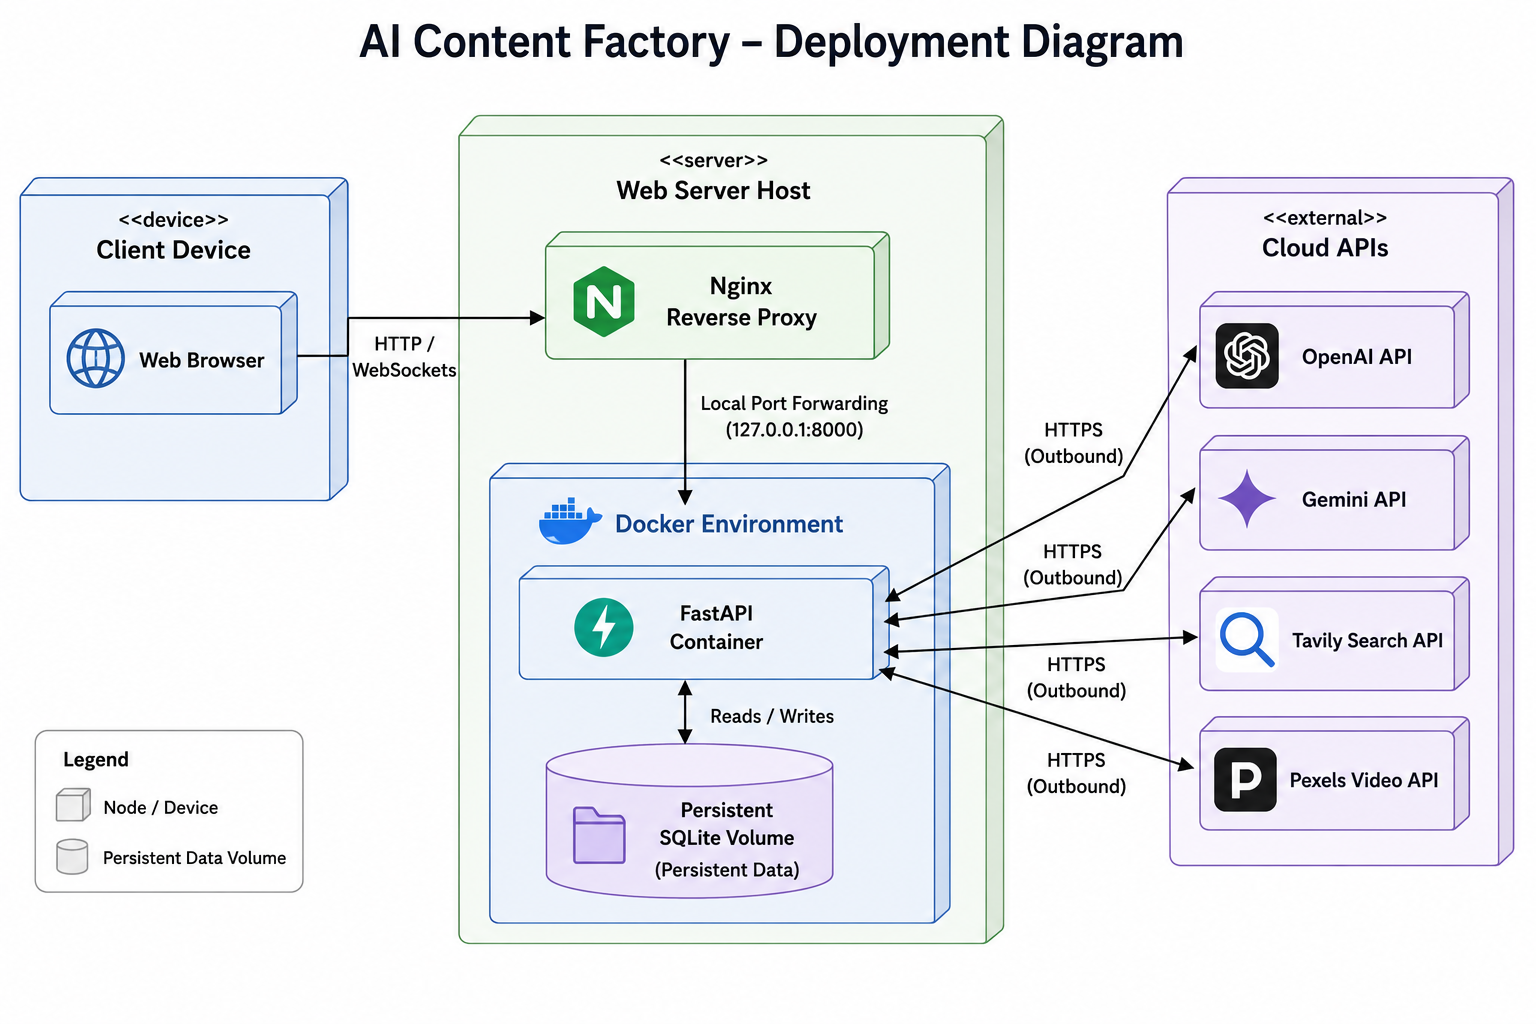
\includegraphics[width=1.0\textwidth, height = 0.75\textheight,keepaspectratio]{Deployment Diagram.png}
	\caption{Logical Deployment and Container Topology of the AI Content Factory}
	\label{fig: Deployment Diagram}
\end{figure}

As shown, the deployment topology consists of:
\begin{itemize}
    \item \textbf{Client Node (Web Browser):} Runs on the user's local machine, rendering the React application and connecting to the backend via HTTP and WebSockets.
    \item \textbf{Reverse Proxy Server (Nginx):} Intercepts incoming requests, manages SSL encryption, serves cached frontend files, and routes API/WebSocket traffic to the backend application container.
    \item \textbf{Application Node (FastAPI Docker Container):} Executes backend processes, including the LangGraph workflow, FastAPI routing engines, and MoviePy compilers.
    \item \textbf{Storage Node (SQLite Database Volume):} A persistent volume on the host server that stores SQLite database checkpoints and execution statistics.
    \item \textbf{External API Services:} Outbound HTTPS connections to OpenAI, Google Cloud, Tavily, and Pexels.
\end{itemize}

\section{Application, Educational Aspects, and Future Directions}

The AI Content Factory has significant practical utility, educational value, and potential for future expansion.

\subsection{Application Areas}
The system serves as a powerful automation tool in several key areas:
\begin{itemize}
    \item \textbf{Automated Marketing Pipelines:} Marketing teams can generate search-engine-optimized blog posts, social media promotional threads (LinkedIn, Twitter), and short promotional videos from a single dashboard.
    \item \textbf{Research and Document Synthesis:} Researchers can upload complex PDFs, docx manuals, or text articles, using the Advanced RAG engine to automatically summarize findings and output structured evidence audits.
    \item \textbf{Multi-Channel Media Production:} Content creators can record solo podcasts and compose subtitled videos simultaneously, eliminating manual editing and timing synchronization tasks.
\end{itemize}

\subsection{Educational Aspects}
From an educational standpoint, this project serves as a reference implementation for advanced computer science concepts:
\begin{itemize}
    \item \textbf{Stateful Software Systems:} Demonstrating how to use LangGraph's checkpointer model to construct reliable, crash-resilient asynchronous applications.
    \item \textbf{Academic G-Eval Auditing:} Showing how to integrate automated academic evaluation frameworks (DeepEval) directly into software pipelines.
    \item \textbf{Multi-Agent Coordination:} Serving as a template for modeling complex parallel writing, reduction, and revision loops in cooperative agent systems.
\end{itemize}

\section{Known Limitations}

The boundaries of the delivered system are stated explicitly below. Each is a
consequence of a deliberate scoping decision rather than an oversight, and each
is accompanied by the mitigation that would be required to remove it.

\begin{itemize}
    \item \textbf{Prompt injection is not mitigated.} Text scraped from the open
      web and text extracted from uploaded documents is inserted into model
      prompts as evidence without any instruction-hierarchy defence --- there is
      no delimiter fencing, no escaping, and no check that an extracted
      ``fact'' originated in the source material rather than in an
      instruction embedded within it. A retrieved page containing adversarial
      text is therefore presented to the extraction model as ordinary content.
      The exposed paths are the research extractor, the document-chunk
      extractor, the section writers, and the quality-assurance auditor.
      Mitigation would require fencing untrusted spans within explicit
      delimiters, instructing the extractor to treat those spans strictly as
      data, and validating that each extracted snippet appears verbatim in its
      source. This is the most significant unaddressed security weakness in the
      system and is documented here rather than deferred silently.

    \item \textbf{Single-worker concurrency.} Human-in-the-loop approval state
      is held in process memory, and an awaiting-approval job blocks a worker
      thread for up to twenty minutes. The API must therefore run as a single
      worker; a multi-replica deployment would require an external task queue
      and a shared approval store. The checkpointer is what makes crash
      recovery possible without one.

    \item \textbf{Access control is a single shared secret.} Setting
      \texttt{API\_KEY} gates every REST route and the WebSocket, but there are
      no per-user accounts and no per-job ownership: any authorised caller can
      read and delete every job. No endpoint is rate limited, and because job
      creation triggers billable third-party API calls, an ungated public
      instance could be driven into unbounded cost.

    \item \textbf{Evaluation scale and independence.} Quality figures come from
      three topics with a single run each, judged by the same model family that
      produced the text, with no baseline comparison arm and no human
      annotation of factual accuracy. Section \ref{sec:threats} discusses these
      constraints in detail.

    \item \textbf{Single-speaker audio.} The podcast studio synthesises one
      Gemini voice; conversational two-speaker output is not implemented.
\end{itemize}

\section{Future Directions}

While the current implementation of the AI Content Factory is robust, several features have been identified for future exploration:

\begin{itemize}
    \item \textbf{Injection-Resistant Retrieval:} Fencing all retrieved and uploaded content within explicit delimiters, instructing extraction models to treat those spans strictly as data, and verifying that every extracted evidence snippet appears verbatim in its source document before it is allowed to reach a writing agent.
    \item \textbf{Graph-Native Human-in-the-Loop:} Replacing the current out-of-graph approval mechanism with LangGraph's own \texttt{interrupt()} and \texttt{Command(resume=...)} primitives, which would move approval state into the checkpointer and remove the single-worker deployment constraint entirely.
    \item \textbf{Distributed Checkpointing with PGVector:} The PostgreSQL checkpointer is already implemented and selected automatically when \texttt{DATABASE\_URL} designates a Postgres instance. The remaining work is to consolidate the separate ChromaDB vector store into the same database using \textbf{PGVector}, so that graph state and semantic embeddings share one transactional backend rather than two independently failing services.
    \item \textbf{Multi-Speaker Podcasts:} Upgrading the Gemini Podcast Studio to generate two-speaker scripts, leveraging distinct native voices (e.g., Aoede and Charon) to simulate natural interview dynamics.
    \item \textbf{Custom Video Overlay Templates:} Integrating support for custom CSS video layout transitions, localized image overlays, and human-like avatar overlays in MoviePy video renders.
    \item \textbf{Local Fine-Tuned LLMs:} Adding configurations to support running local, fine-tuned open-source models (such as LLaMA-3 or Mistral) via Ollama, reducing API cost dependencies on proprietary third-party engines.
\end{itemize}